\chapter{Razvijena programska potpora}

\section{Struktura programske potpore}
Na slici \ref{fig:uml} prikazana je struktura razvijene programske potpore u obliku UML dijagrama razreda. U nastavku poglavlja bit će detaljnije opisani upravljački programi za sklopove ADS131M08 i ADT7301, kao i funkcije za prikupljanje i obradu podataka u modulu \textit{Sensor Board}.

\begin{figure}[h!]
    \centering
    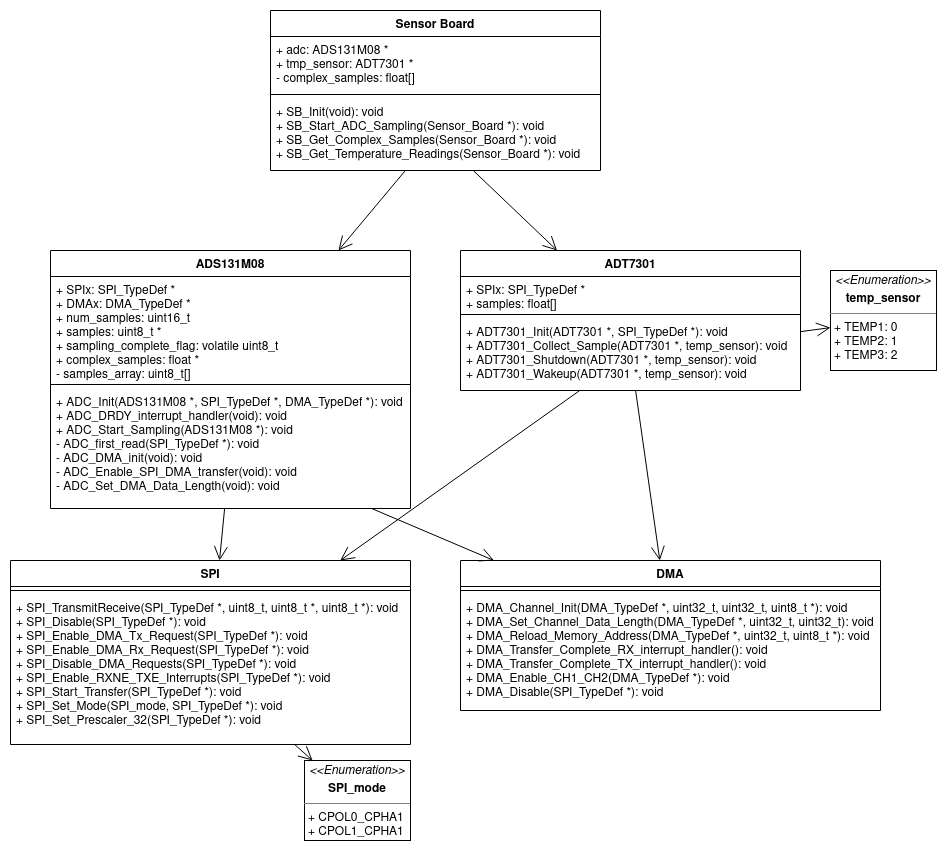
\includegraphics[width=\textwidth]{slike/uml.png}
    \caption{Prikaz strukture programske potpore UML dijagramom razreda}
    \label{fig:uml}
\end{figure}

\section{Korištene biblioteke i alati}
Tvrtka ST Microelectronics nudi dva skupa programskih biblioteka za razvoj programske potpore namijenjene njihovim mikrokontrolerima: \textit{Hardware Abstraction Layer} (HAL) i \textit{Low Level} (LL) biblioteke. HAL biblioteke nude višu razinu apstrakcije sklopovlja od LL biblioteka, što omogućuje jednostavniji i brži razvoj, te olakšanu prenosivost između različitih mikrokontrolera istog proizvođača. S druge strane, LL biblioteke nude vrlo nisku razinu apstrakcije, što zahtijeva vrlo dobro poznavanje strukture i načina rada mikrokontrolera od strane programera, ali zato omogućuje pisanje programa koji zauzimaju vrlo malu količinu memorije \cite{stm_hal_ll}. Također, korištenje LL biblioteka smanjuje ukupno vrijeme izvođenja jer se eliminiraju česte provjere parametara funkcija ugrađene u HAL biblioteke. Upravo zbog vrlo ograničenih resursa dostupnih na odabranom mikrokontroleru, tijekom razvoja programske potpore opisane u radu \cite{diplomski_goran_petrak} donesena je odluka o korištenju LL biblioteka. Iz tog razloga LL biblioteke korištene su i u razvoju programske potpore opisane u ovom radu.

Programska potpora razvijena je u programskom jeziku C, uz korištenje prevoditelja GCC u sklopu \textit{GNU ARM Embedded Toolchain} paketa. Za razvoj je korišteno razvojno okruženje STM32CubeIDE, s integriranim alatom CubeMX. Navedeni alat omogućuje automatsko generiranje programskog koda za inicijalizaciju periferija mikrokontrolera i jednostavnu konfiguraciju signala takta kroz grafičko sučelje.

\section{Upravljački program za AD pretvornik ADS131M08}

Zadaća upravljačkog programa za ADS131M08 je prikupiti rezultate AD pretvorbe putem SPI sučelja. Zbog velike količine podataka koje je potrebno prikupiti, za prijenos podataka između SPI periferije i memorije koristi se DMA sklop. Upravljački su programi pisani tako da budu neovisni o bilo kakvoj programskoj logici više razine, pa ih je moguće ponovno iskoristiti u budućim nadogradnjama programske potpore ili u drugim projektima. Funkcionalnost programa ostvarena je pomoću tri glavne funkcije:

\begin{lstlisting}
void ADC_Init(ADS131M08 *adc_struct, SPI_TypeDef *SPIx, DMA_TypeDef *DMAx);
void ADC_Start_Sampling(ADS131M08 *adc);
void ADC_DRDY_interrupt_handler();
\end{lstlisting}

Također, definirana je i struktura \texttt{ADS131M08} preko koje se razmjenjuju konfiguracijski podaci između pozivajućeg modula i upravljačkog programa, te čuvaju pokazivači na prikupljene podatke:

\begin{lstlisting}
typedef struct {
    SPI_TypeDef *SPIx;
    DMA_TypeDef *DMAx;
    uint16_t num_samples;
    uint8_t *samples;
    volatile uint8_t sampling_complete_flag;
    float *complex_samples;
} ADS131M08;
\end{lstlisting}

Funkcija \texttt{ADC\_Init} inicijalizira članove strukture \texttt{ADS131M08}, postavlja parametre SPI komunikacije tako da odgovaraju onima koje podržava sklop ADS131M08, i poziva pomoćnu funkciju \texttt{ADC\_DMA\_Init} postavlja izvorišnu i odredišnu adresu DMA prijenosa i omogućuje DMA prekide.

Nakon što je inicijalizacija dovršena, dohvaćanje podataka može se pokrenuti funkcijom \texttt{ADC\_Start\_Sampling}. Ova funkcija prvo poziva pomoćnu funkciju \texttt{ADC\_First\_Read} koja obavlja čišćenje međuspremnika ADC-a s dva uzastopna čitanja kao što je opisano u potpoglavlju \ref{section_adc}. Zatim se omogućuje prekid kojeg izaziva padajući brid signala na \textoverline{DRDY} priključku ADC-a, čime započinje prikupljanje podataka.

Prekidna rutina koja rukuje navedenim prekidom (prekid je doveden na prekidnu liniju EXTI4) poziva funkciju \texttt{ADC\_DRDY\_interrupt\_handler}. Funkcija postavlja duljinu prijenosa i odredišnu adresu, omogućuje DMA prijenos pozivanjem funkcija koje postavljaju odgovarajuće bitove u registrima SPI i DMA periferija, te postavlja \textoverline{CS} priključak ADC-a u nisku logičku razinu. Nakon toga SPI prijenos se odvija automatski sklopovskom sinkronizacijom između SPI i DMA periferija. Po završetku zadanog broja prijenosa onemogućuje se \textoverline{DRDY} prekid.

Podaci prikupljeni s ADC-a spremaju se u statički alocirano polje 8-bitnih cijelih brojeva. Jedan uzorak svakog od kanala veličine je 24 bita, odnosno 3 bajta. Ukupna duljina podataka jednog okvira, koji sadrži uzorke svih 8 kanala, ispis statusnog registra ADC-a i CRC zaštitni kod poruke, je 30 bajtova. Prikuplja se 256 okvira, pa ukupna duljina podataka iznosi 7680 bajtova.

\section{Upravljački program za temperaturni senzor ADT7301}

Upravljački program za temperaturni senzor prikuplja uzorke temperature od senzora ADT7301. Razvijene su četiri funkcije za rad sa senzorom:

\begin{lstlisting}
void ADT7301_Init(ADT7301 *adt7301_struct, SPI_TypeDef *SPIx);
void ADT7301_Collect_Sample(ADT7301 *adt7301, temp_sensor ts);
void ADT7301_Shutdown(ADT7301 *adt7301, temp_sensor ts);
void ADT7301_Wakeup(ADT7301 *adt7301, temp_sensor ts);
\end{lstlisting}

Na senzorskoj pločici nalaze se tri temperaturna senzora, pa zato funkcije za prikupljanje podataka primaju parametar \texttt{ts} koji označava s kojeg senzora treba prikupiti podatak. Parametar je enumeracijskog tipa \texttt{temp\_sensor}:

\begin{lstlisting}
typedef enum {
    TEMP1 = 0,
    TEMP2 = 1,
    TEMP3 = 2
} temp_sensor;
\end{lstlisting}

Slično kao i kod upravljačkog programa za AD pretvornik, parametri i prikupljeni podaci čuvaju se u strukturi ADT7301:

\begin{lstlisting}
typedef struct {
	SPI_TypeDef *SPIx;
	float samples[3];
} ADT7301;
\end{lstlisting}

Funkcija \texttt{ADT7301\_Init} inicijalizira članove strukture \texttt{ADT7301} i postavlja SPI komunikaciju. Ostale tri funkcije imaju međusobno sličnu funkcionalnost - šalju i primaju dva bajta podataka s odabranog temperaturnog senzora korištenjem funkcije \texttt{SPI\_TransmitReceive}. 

Funkcija \texttt{ADT7301\_Collect\_Sample} obavlja pretvorbu primljenog podatka u stvarnu vrijednost temperature (iskazanu u \textcelsius{}) u formatu realnog broja s pomičnim zarezom, i zapisuje vrijednost u polje \texttt{samples} strukture \texttt{ADT7301}. Mjesto u polju na kojeg će biti zapisana vrijednost ovisi o odabranom senzoru \texttt{ts} (indeks 0, 1 ili 2).

Funkcija \texttt{ADT7301\_Shutdown} šalje naredbu za postavljanje senzora u način rada niske potrošnje (\textit{shutdown}). Podatak primljen sa senzora zanemaruje se.

Funkcija \texttt{ADT7301\_Wakeup} "budi" senzor iz načina rada niske potrošnje. Primljeni podatak također se zanemaruje.

Za SPI komunikaciju s temperaturnim senzorima koristi se bitno manja frekvencija takta nego za komunikaciju s AD pretvornikom. Djelitelj signala takta postavljen je na vrijednost 32, što s frekvencijom takta sabirnice APB1 od 20 MHz daje frekvenciju SPI takta od 625 kHz. Razlog tome je što je tijekom uhodavanja primijećeno da pri većim frekvencijama dolazi do značajnog deformiranja signala takta. Nije utvrđeno zašto se to događa pri komunikaciji s temperaturnim senzorima, a ne događa se pri komunikaciji s ADC-om. Prema podacima iz dokumentacije senzora, maksimalna frekvencija SPI takta iznosi 20 MHz, no zbog navedenih izobličenja nije bilo moguće postići tu frekvenciju i osigurati ispravan rad.


\section{Programska potpora za prikupljanje i obradu podataka} \label{obrada}

Programska potpora za prikupljanje i obradu podataka senzorskog podsustava grupirana je u modul \texttt{sensor\_board}. Omogućuje prikupljanje podataka korištenjem prethodno opisanih upravljačkih programa za sklopove ADS131M08 i ADT7301, te priprema podatke o svjetlosnom onečišćenju prikupljene s ADC-a za obradu algoritmom \textit{Fast Fourier Transform} (FFT).

Za prikupljanje podataka razvijene su sljedeće funkcije:
\begin{lstlisting}
void SB_Init(Sensor_Board *sb);
void SB_Start_ADC_Sampling(Sensor_Board *sb);
void SB_Get_Temperature_Readings(Sensor_Board *sb);
\end{lstlisting}

Funkcija \texttt{SB\_Init} inicijalizira strukturu \texttt{Sensor\_Board}, koja enkapsulira strukture \texttt{ADS131M08} i \texttt{ADT7301}:
\begin{lstlisting}
typedef struct {
    ADS131M08 *adc;
    ADT7301 *tmp_sensor;
} Sensor_Board;
\end{lstlisting}

Funkcija \texttt{SB\_Start\_ADC\_Sampling} inicijalizira ADC, a zatim pokreće postupak dohvaćanja uzoraka s ADC-a pozivom funkcije \texttt{ADC\_Start\_Sampling}. Funkcija je neblokirajuća, dakle moguće je obavljati druge zadatke za vrijeme dohvaćanja uzoraka.

Za dohvaćanje podataka s temperaturnih senzora namijenjena je funkcija \\\texttt{SB\_Get\_Temperature\_Readings}. Funkcija inicijalizira temperaturne senzore, a zatim svaki od tri senzora prvo "budi" iz \textit{shtdown} načina rada, prikuplja uzorak temperature sa senzora i vraća ga u \textit{shutdown} način rada.

Kako bi se iz podataka dobivenih od fotodetektora mogla dobiti informacija o spektralnoj gustoći svjetla sa Zemlje, potrebno je izvršiti određenu obradu podataka. Prvi je korak u toj obradi računanje spektra diskretnog signala algoritmom FFT. Uzastopni uzorci s jednog fotodetektora, odnosno uzorci s jednog kanala ADC-a, promatraju se kao vremenski niz, tj. diskretni signal u vremenskoj domeni. Uzima se 256 uzoraka svakog kanala kako bi se mogla izračunati transformacija u 256 točaka. To je najveći broj uzoraka koji se može prikupiti s obzirom na ograničenja memorije\footnote{Da bi FFT algoritam radio efikasno, broj uzoraka treba biti potencija broja 2. Za računanje FFT u 512 točaka potrebno je više radne memorije nego što je dostupno na odabranom mikrokontroleru, pa se zato računa FFT u 256 točaka.}. Za računanje FFT koristi se implementacija iz CMSIS (\textit{Cortex Microcontroller Software Interface Standard Digital Signal Processing}) DSP (\textit{Digital Signal Processing}) biblioteke. Ova biblioteka pruža programsko sučelje za korištenje algoritama za digitalnu obradu signala koji su posebno optimirani za izvođenje na procesorskim jezgrama Cortex-M koje proizvodi tvrtka Arm \cite{cmsis_dsp_documentation}.

Funkcija iz CMSIS DSP biblioteke koja implementira brzu Fourierovu transformaciju nad realnim nizovima 32-bitnih brojeva s pomičnim zarezom ima sljedeću deklaraciju:

\begin{lstlisting}
void arm_rfft_fast_f32( const arm_rfft_fast_instance_f32 *S,
                        float32_t *p,
                        float32_t *pOut,
                        uint8_t ifftFlag );	
\end{lstlisting}

Parametar \texttt{S} je struktura s konfiguracijskim podacima za algoritam (između ostalog sadrži i duljinu niza), \texttt{p} je pokazivač na ulazni niz, \texttt{pOut} je pokazivač na izlazni niz, a \texttt{ifftFlag} je zastavica koja označava radi li se o inverznoj transformaciji.

Navedena funkcija, iako radi s realnim ulaznim nizovima (pa se taj algoritam još naziva i \textit{Real Fast Fourier Transform} - RFFT), brza Fourierova transformacija definirana je nad kompleksnim brojevima (\textit{Complex Fast Fourier Transform} - CFFT). Zato se polje s ulaznim nizom mora formatirati na način da se svaki podatak prikazuje kao zbroj svoje realne i imaginarne vrijednosti. Primjerice, formatirano polje s N ulaznih podataka simbolički možemo prikazati na sljedeći način, gdje \texttt{real[i]} označava realnu vrijednost podatka s rednim brojem \texttt{i}, a \texttt{imag[i]} njegovu imaginarnu vrijednost:

\begin{lstlisting}
[real[0], imag[0], real[1], imag[1], ..., real[N-1], imag[N-1]]
\end{lstlisting}

Izlazno je polje formatirano na isti način. No, zbog svojstva simetrije spektra realnih signala, druga polovica spektra u potpunosti je određena prvom polovicom. Za takve signale, realni dio spektra je parna funkcija, a imaginarni dio neparna, pa se svaki uzorak druge polovice spektra može prikazati kao konjugirano-kompleksna vrijednost odgovarajućeg uzorka iz prve polovice \cite{petkovic_oos}. Zato je spektar signala duljine N uzoraka moguće u prikazati s $\frac{N}{2} + 1$ kompleksnih brojeva. Osim toga, prvi i posljednji od tih brojeva su čisto realni, pa se oni prikazuju kao prva dva elementa izlaznog polja. Zato izlazno polje ima dvostruko manju duljinu od ulaznog, i može se prikazati u obliku:

\begin{lstlisting}
[real[0],real[N/2],real[1],imag[1],...,real[N/2-1],imag[N/2-1]]
\end{lstlisting}

FFT obrada signala zahtijeva znatnu količinu procesorskih resursa, pa će se zato obavljati u vremenu kada su ostali sustavi korisnog tereta satelita neaktivni \engl{downtime}, a programski će za nju biti zadužen zadatak neovisan od zadatka za upravljanje senzorskim podsustavom. U okviru ovog rada realizirano je poravnanje podataka dobivenih s ADC-a tako da oni budu u obliku pogodnom za korištenje kao ulazno polje funkcije \texttt{arm\_rfft\_fast\_f32}, i zapisivanje takvih podataka u trajnu memoriju \engl{non-volatile memory}. Program za obradu podataka tada može jednostavno učitati podatke iz trajne memorije, provesti FFT transformaciju i ostalu obradu koja slijedi nakon nje, i zapisati rezultate natrag u trajnu memoriju.

Formatiranje podataka u polje kompleksnih realnih brojeva s pomičnim zarezom ostvaruje sljedeća funkcija:

\begin{lstlisting}
void SB_Get_Complex_Samples(Sensor_Board *sb);
\end{lstlisting}

Funkcija pretvara 24-bitne rezultate AD pretvorbe u 16-bitne (vodeći računa da se preskoče nepotrebni podaci dobiveni s ADC-a kao što je ispis statusnog registra), zatim ih pretvara u stvarne vrijednosti napona s obzirom na referentni napon ADC-a i zapisuje ih u izlazno polje kao kompleksne brojeve s imaginarnim dijelom jednakim 0. Izlazno polje je statički alocirano i veličine je 16 384 bajta, a u njemu se nakon poziva funkcije nalaze redom uzorci sa svih 8 fotodetektora (prvo 256 kompleksnih uzoraka s kanala 0, zatim 256 kompleksnih uzoraka s kanala 1, itd.).

\section{Integracija s operacijskim sustavom FreeRTOS}

Razvijena programska potpora za upravljanje senzorskim podsustavom integrirana je s cjelokupnom programskom potporom PDH računala. Programska potpora koristi operacijski sustav za rad u stvarnom vremenu FreeRTOS. Raspodjela poslova u FreeRTOS-u obavlja se korištenjem takozvanih zadataka \engl{tasks}. Programska potpora PDH računala podijeljena je na 4 zadatka, koji su ovdje navedeni redom od zadatka s najvišim prioritetom do zadatka s najnižim prioritetom \cite{diplomski_goran_petrak}:

\begin{description}
    \item[Interpreter Task:] komunicira s CDH računalom, odnosno osobnim računalom u demonstracijskoj inačici programa, i postavlja parametre za izvršavanje ostalih zadataka (\textit{device tasks}),
    \item[X-band and Storage Management Task:] upravlja komunikacijskim podsustavom i datotečnim sustavom za trajnu memoriju,
    \item[Camera Task:] upravlja radom kamere,
    \item[Sensor Board Task:] upravlja senzorskim podsustavom.
\end{description}

\begin{figure}[htb]
    \centering
    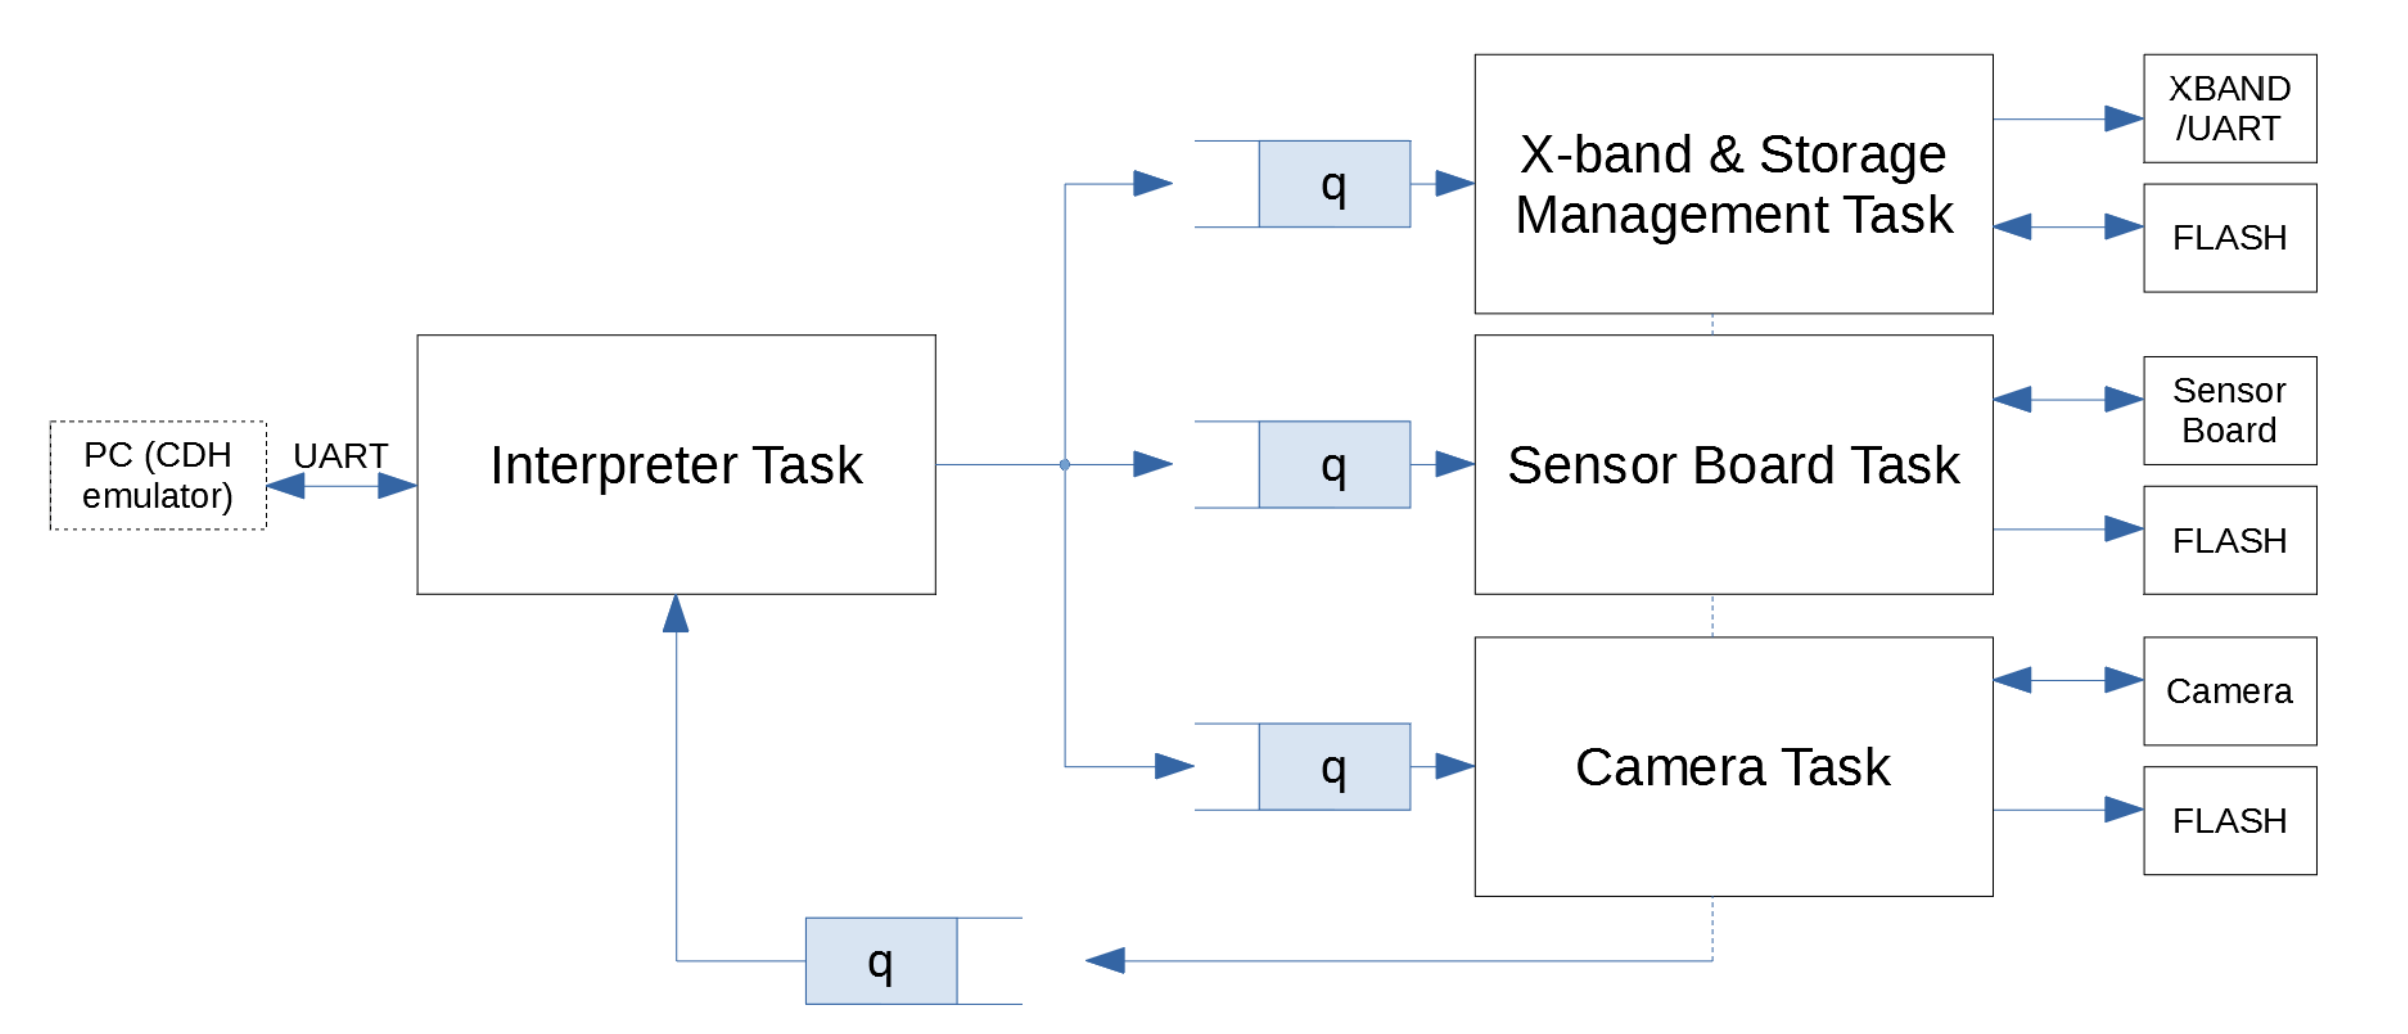
\includegraphics[width=\textwidth]{slike/rtos_zadaci.png}
    \caption{Zadaci programske potpore PDH računala \cite{diplomski_goran_petrak}.}
    \label{fig:rtos_zadaci}
\end{figure}

Zadaci međusobno komuniciraju putem redova poruka \engl{message queue}. Zadatak Interpreter postavlja parametre za svaki od \textit{device} zadataka (npr. ime datoteke u koju se podaci spremaju, duljinu ekspozicije kamere, itd.) te postavlja poruku s parametrima u red poruka odgovarajućeg zadatka. Kada su postavljeni parametri za sve zadatke, zadatak Interpreter spušta svoj prioritet na najniži u sustavu. To omogućuje deblokadu ostalih zadataka, koji čitaju poruke iz pripadajućih redova i obavljaju svoje poslove. Nakon što neki od zadataka završi s poslom, šalje poruku o uspješnosti u red poruka zadatka Interpreter, te zatim biva blokiran čekajući na poruku iz (sada praznog) reda poruka. Kada svi zadaci obave svoj posao, ponovno se aktivira zadatak Interpreter i ciklus se ponavlja. Komunikacija između zadataka prikazana je slikom \ref{fig:rtos_zadaci}. Eventualni dijeljeni resursi ne štite se nikakvim posebnim mehanizmima jer je sustav zamišljen tako da se zadaci međusobno ne prekidaju.

U sklopu rada \cite{diplomski_goran_petrak} razvijen je i datotečni sustav za trajnu \textit{Flash} memoriju koja se nalazi na tiskanoj pločici PDH računala. Za rad s datotečnim sustavom razvijene su korisničke funkcije po uzoru na standard POSIX (\textit{Portable Operating System Interface}). Funkcije omogućuju jednostavno pisanje i čitanje datoteka s \textit{Flash} memorije, te se koriste u svim \textit{device} zadacima.

U sklopu ovog rada razvijen je zadatak Sensor Board Task. Putem zadatka Interpreter korisnik može zadati imena datoteka u koje će se spremiti uzorci sa fotosenzora (u kompleksnom zapisu, kao što je opisano u potpoglavlju \ref{obrada}) i uzorci s temperaturnih senzora. Imena datoteka su cijeli brojevi u intervalu od 0 do 1023. Nakon što se parametri pročitaju iz reda poruka, pokreće se postupak prikupljanja podataka:

\begin{lstlisting}
Sensor_Board sb;
SB_Init(&sb);
SB_Get_Temperature_Readings(&sb);
SB_Start_ADC_Sampling(&sb);
SB_Get_Complex_Samples(&sb);
\end{lstlisting}

Po završetku izvođenja ovog odsječka programskog koda, uzorcima fotosenzora može se pristupiti preko pokazivača \texttt{adc->complex\_samples} u strukturi \texttt{sb}, a uzorcima temperaturnih senzora preko pokazivača \texttt{tmp\_sensor->samples}, također u strukturi \texttt{sb}. Prikupljeni podaci zapisuju se u datotečni sustav u datotekama čija su imena zadana parametrima zadataka, korištenjem prethodno spomenutih POSIX funkcija. Za potrebe demonstracije dodan je i ispis prikupljenih podataka putem sučelja UART (\textit{Universal Asynchronous Receiver Transmitter}).

\subsection{Mapiranje dijelova memorije u RAM2}

Memorija potrebna za izvršavanje zadatka Sensor Board Task iznosi približno 23.5 kB. Najveći dio te memorije zauzima polje s kompleksnim uzorcima fotosenzora (oko 16 kB) i polje s primljenim podacima s ADC-a (oko 7.5 kB). Prije integracije programske potpore za upravljanje senzorskim podsustavom, količina slobodne memorije u primarnoj RAM memoriji aplikacije PDH računala iznosila je svega 3.8 kB, što nije ni približno dovoljno za spremanje svih potrebnih podataka. No, mikrokontroler STM32L471VGT6 ima i sekundarnu RAM memoriju naziva RAM2 \cite{stm32l4_manual}. Ta je memorija kapaciteta 32 kB i mapirana je na adrese memorijskog prostora od 0x10000000 do 0x10008000.

Prema početnim postavkama programa povezivača \engl{linker} koje definira proizvođač mikrokontrolera u \textit{linker} skripti \texttt{STM32L471VGTX\_FLASH.ld}, sve statički alocirane varijable smještaju se u memorijsku sekciju \texttt{.bss} memorije RAM. U navedenoj \textit{linker} skripti definirana je i memorija RAM2, međutim nije joj dodijeljena nijedna memorijska sekcija. Kako bi se kreirala memorijska sekcija u koju će se spremati podaci čije će memorijske adrese biti mapirane na adrese pridijeljene memoriji RAM2, potrebno je u \textit{linker} skriptu dodati sljedeći odsječak koda:

\begin{lstlisting}
SECTIONS
{
    .ram2 :
    {
        KEEP(*(.ram2))
    } >RAM2

    /* ... ostatak koda linker skripte ... */
\end{lstlisting}

Naredba \texttt{SECTIONS} definira kako se sekcije u ulaznim datotekama programa povezivača trebaju mapirati u izlaznu datoteku \cite{ld_dokumentacija}. Linija 3 gornjeg odsječka definira izlaznu sekciju \texttt{.ram2}. Izraz na liniji 5 znači da se ulazna sekcija \texttt{.ram2} definirana u bilo kojoj ulaznoj datoteci (označeno \textit{wildcard} simbolom \texttt{*}) treba mapirati na adresu izlazne sekcije \texttt{.ram2}. Naredba \texttt{KEEP()} govori programu povezivaču da ulazne sekcije \texttt{*.ram2} ne smije ukloniti tijekom \textit{garbage collection} postupka. Izraz na liniji 6 mapira adresu izlazne sekcije \texttt{.ram2} u memoriju RAM2.

Preostaje još samo signalizirati programu povezivaču koje programske varijable treba smjestiti u sekciju \texttt{.ram2}. To se može postići dodjeljivanjem atributa \texttt{section} varijabli navođenjem izraza \texttt{\_\_attribute\_\_((section(".ram2")))} uz njenu deklaraciju. Radi bolje čitljivosti koda, definiran je makro izraz:

\begin{lstlisting}
#define _SECTION_RAM2 __attribute__((section(".ram2")));
\end{lstlisting}

Makro izraz je zatim naveden uz deklaracije polja u kojima se spremaju kompleksni uzorci fotosenzora i podaci dohvaćeni s ADC-a. Raspored memorije nakon ove modifikacije prikazan je slikom \ref{fig:memorija}.

\begin{figure}[htb]
    \centering
    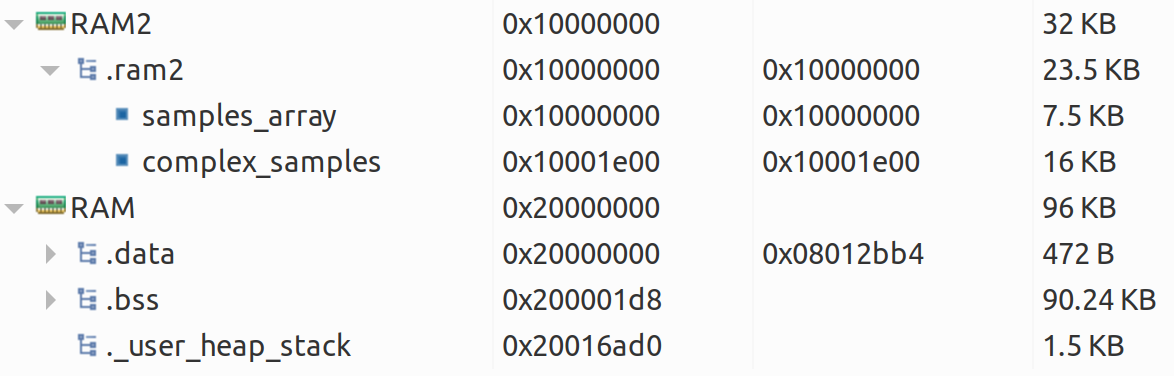
\includegraphics[width=\textwidth]{slike/memorija.png}
    \caption{Raspored memorije nakon smještanja polja \texttt{complex\_samples} i \texttt{samples\_array} u RAM2.}
    \label{fig:memorija}
\end{figure}